\documentclass[12pt]{article}
\usepackage[utf8]{inputenc}
\usepackage{amsmath}
\usepackage{times}
\usepackage{amsfonts}
\usepackage{xcolor}
\usepackage{amssymb}
\usepackage{graphicx}
\usepackage{tabularx}
\usepackage[font=small,labelfont=bf]{caption}
\usepackage[font=small]{subcaption}
\usepackage{wrapfig}
\usepackage[section]{placeins}

\renewcommand{\arraystretch}{1.5}


\begin{document}
\vspace{20mm}

{\LARGE Traveling waves in quasi one-dimensional neuronal minicolumns - supplemental information}

\ \\
{\bf \large Vincent Baker, vjb42@drexel.edu$^{\displaystyle 1}$}\\
{\bf \large Luis Cruz, ccruz@drexel.edu$^{\displaystyle 1}$}\\
{$^{\displaystyle 1}$Drexel University, Department of Physics.}\\

\pagebreak

\subsection*{Model Summary}
\begin{table}[!htb]
 \caption{Model Summary}
 \label{tab:all_params}
 \centering
 \begin{tabular}{c}
  \textbf{Model} \\
  \hline \\
 \end{tabular} \\
 \begin{tabular}{l|l}
  Population & Excitatory, inhibitory \\
  Topology & Small columnar ensemble, Z extents $\gg$ X,Y extents \\
  Connectivity & Stochastic, $P_c$ exponentially decays with distance between neurons \\
  Neuron model & Izhikevich model with distribution of neuron parameters \\
  Synapse response & Exponential synaptic response with randomized peak connection strength  \\
  Spike propagation & Delay proportional to distance, Fixed propagation time \\
  Input & Random input to all neurons, Fixed stimulus to neurons at the bottom of the SCE \\
 \end{tabular}
\end{table}

\clearpage

\subsection*{Wave detection and labeling}
\color{red}
Our automated wave detection and labeling process must find and characterize waves under the varying conditions set by our simulation parameters.
The wave extent, wave speed, and the number of background spikes all depend upon the simulation parameters.
To validate the detection and labeling process we visually inspected the results for a variety of simulations.
Sample visualizations for varying values of $K$ are shown in Figure \ref{fig:detector_test}.
\begin{figure}[!htb]
 \caption{The clustering and wave labeling process. Spike raster plot (left), filtered clusters (middle) and labeled waves (right, each color is a unique wave) are shown for SCE with different values of $K$. }
 \label{fig:detector_test}
 \centering
   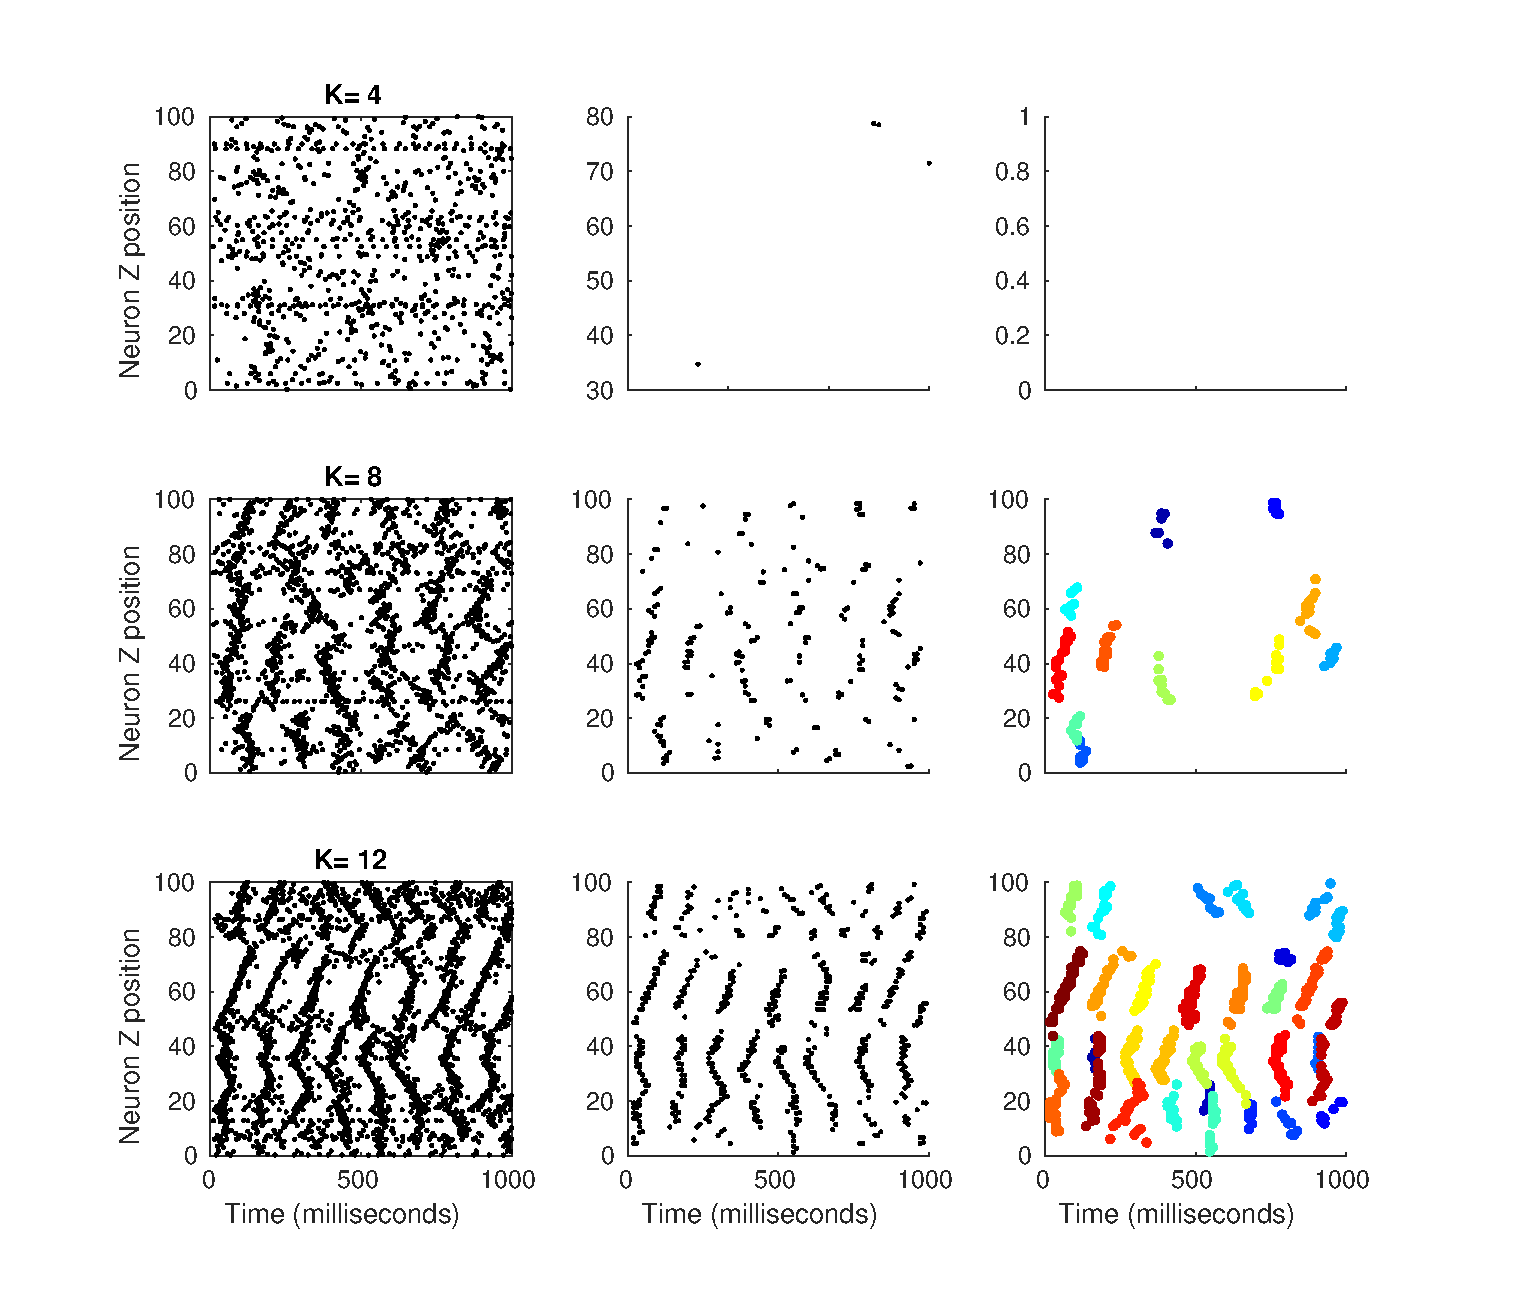
\includegraphics[width=\textwidth]{fig/DetectorTest}
\end{figure}
\FloatBarrier
\color{black}

\clearpage

\color{red}
\subsection*{Additional SCE statistics}
\begin{figure}[!htb]
 \caption{Distribution of (A) number of post-synaptic connections per neuron and (B) delay time. Data was taken over 100 realizations of a 2x2x50 SCE, $\lambda=2.5$, $\kappa=1$.  } 
 \begin{tabular}{c}
     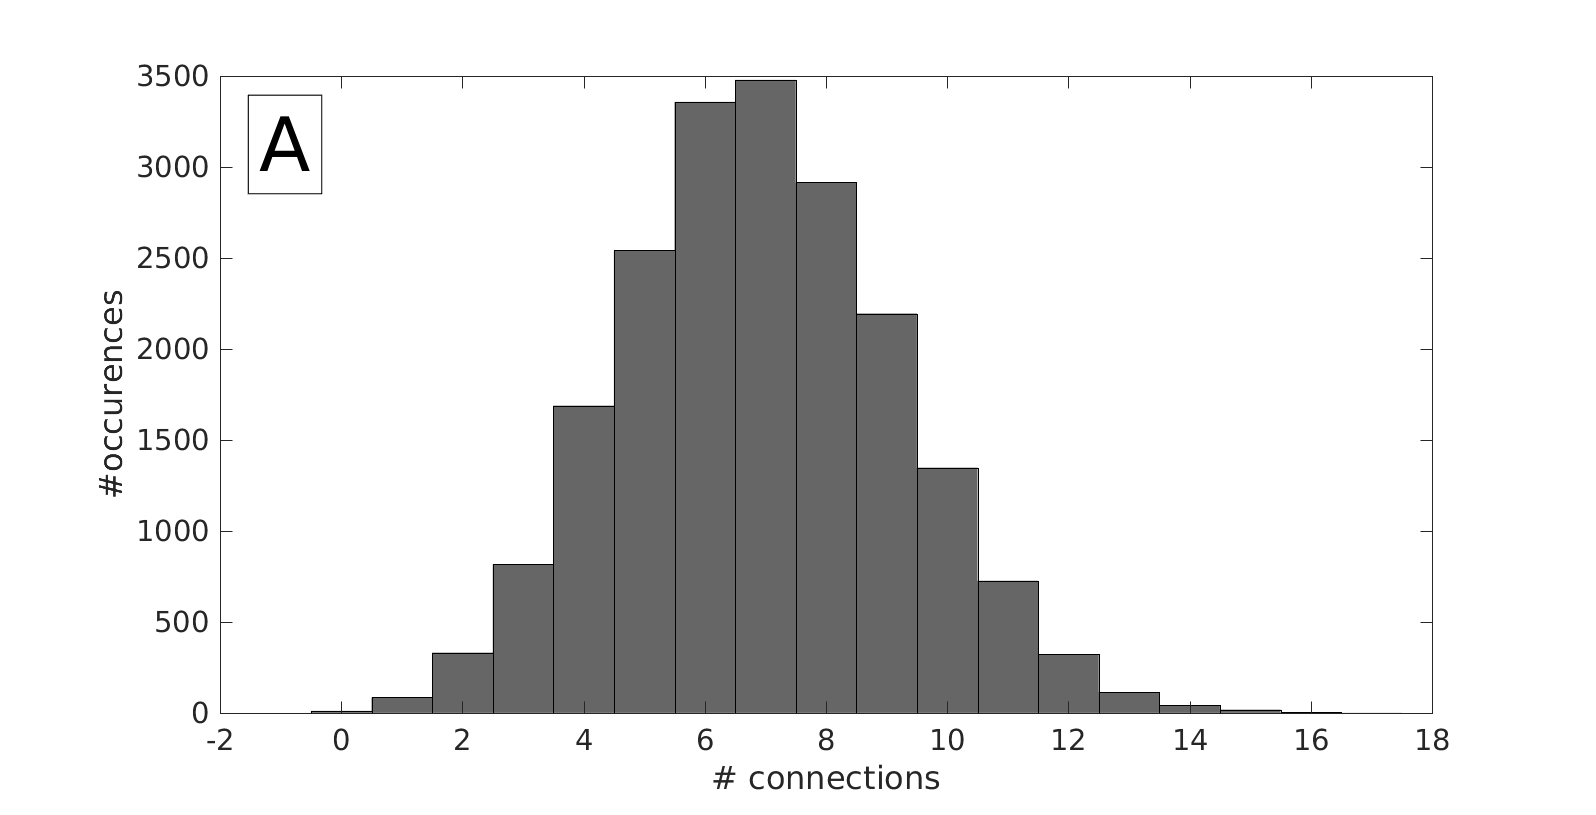
\includegraphics[width=\textwidth]{fig/ConnectionNumberDistribution} \\
     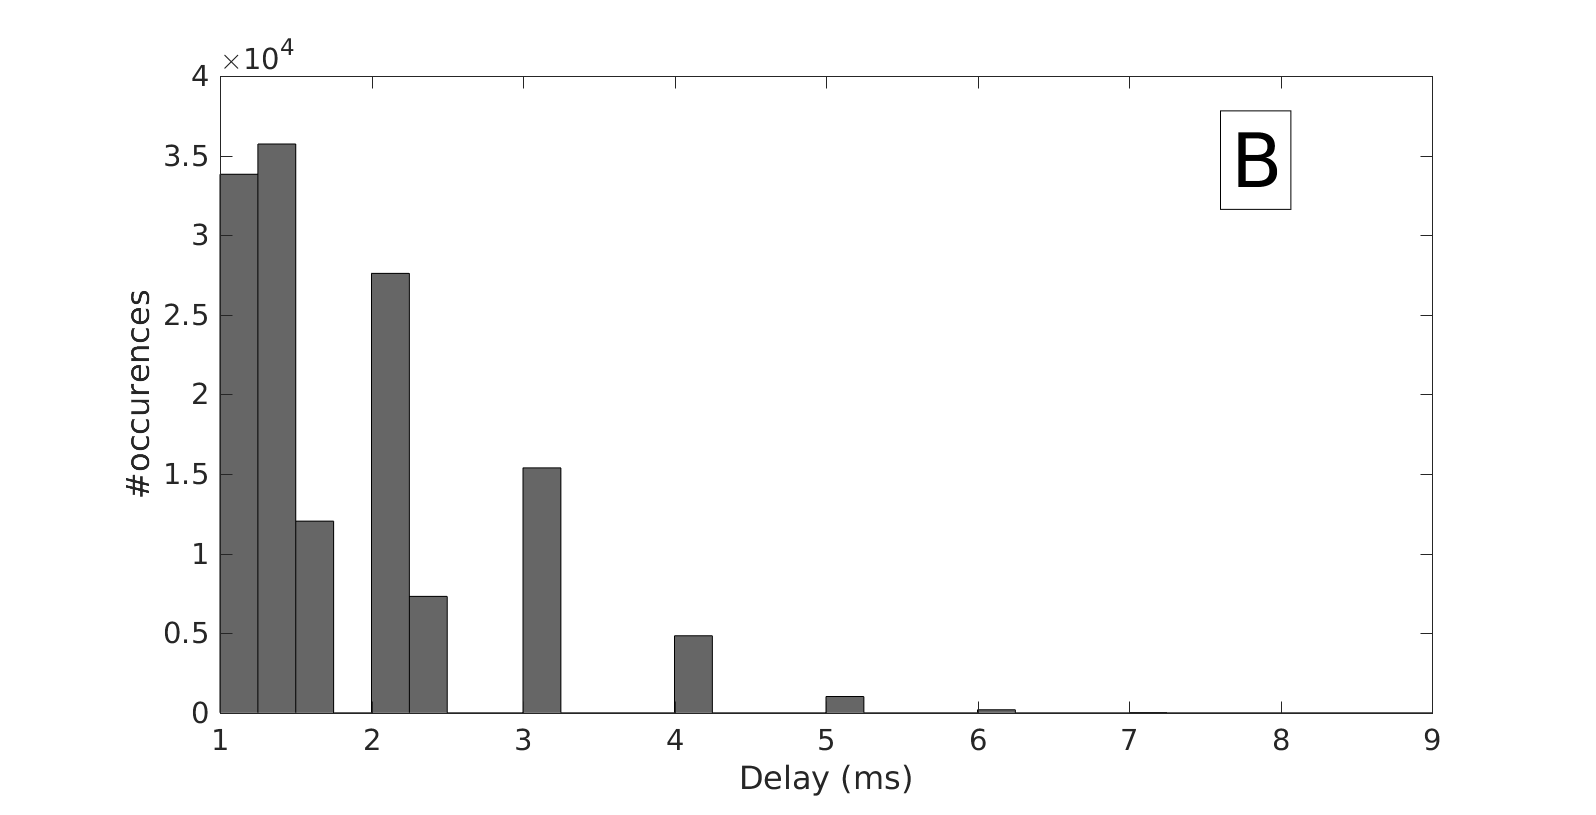
\includegraphics[width=\textwidth]{fig/DelayDistribution} 
 \end{tabular}
\end{figure}
 \FloatBarrier
\color{black}
 
\clearpage
\subsection*{Example FIE and FFE plots}
\begin{figure}[!htb]
 \caption{FIE and FFE for nine example columns. } 
 \begin{tabular}{ccc}
     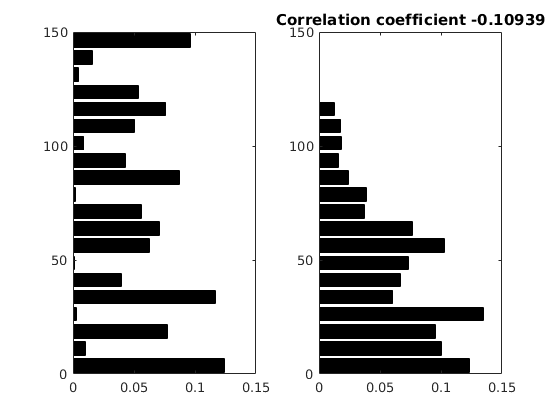
\includegraphics[width=0.3\textwidth]{fig/ccf/ccf1} & 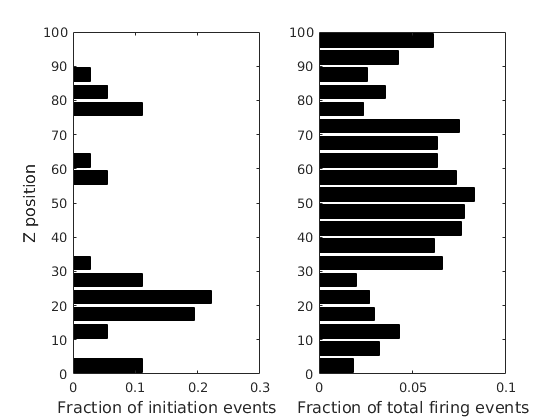
\includegraphics[width=0.3\textwidth]{fig/ccf/ccf2} & 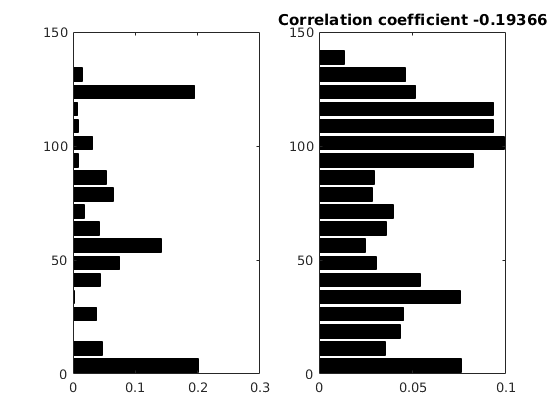
\includegraphics[width=0.3\textwidth]{fig/ccf/ccf3} \\
     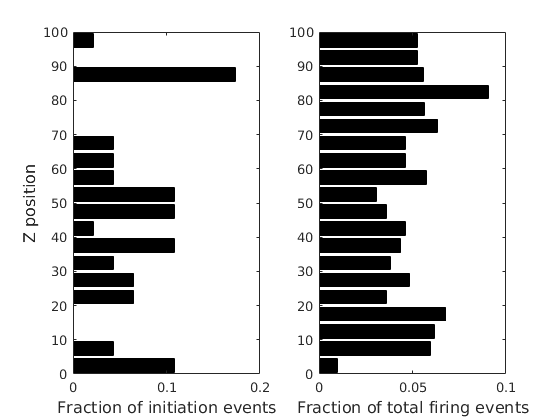
\includegraphics[width=0.3\textwidth]{fig/ccf/ccf4} & 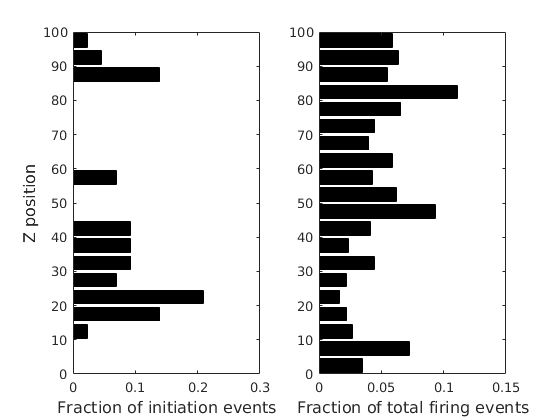
\includegraphics[width=0.3\textwidth]{fig/ccf/ccf5} & 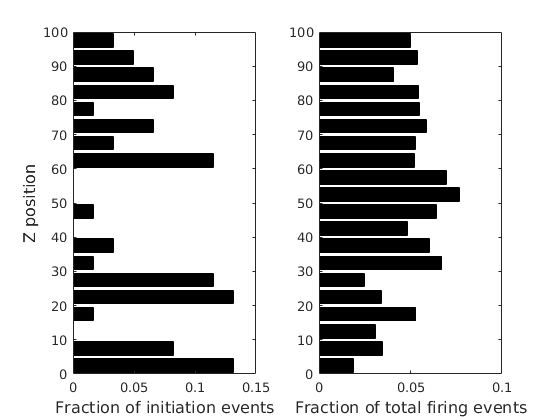
\includegraphics[width=0.3\textwidth]{fig/ccf/ccf6} \\
     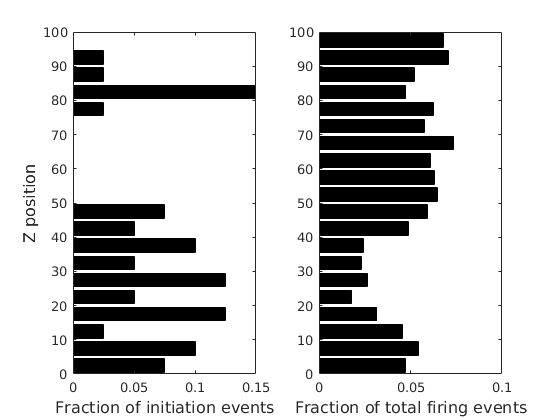
\includegraphics[width=0.3\textwidth]{fig/ccf/ccf7} & 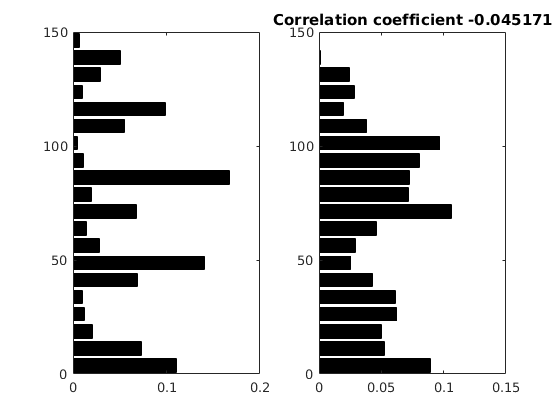
\includegraphics[width=0.3\textwidth]{fig/ccf/ccf8} & 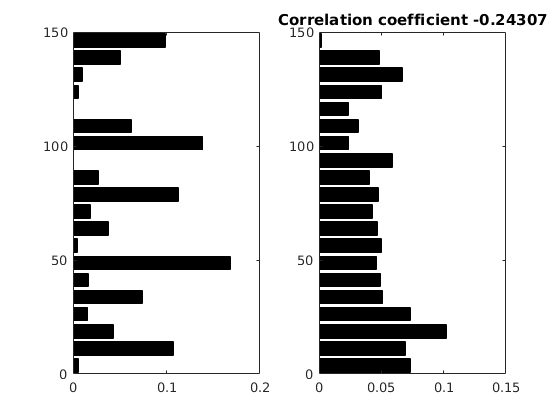
\includegraphics[width=0.3\textwidth]{fig/ccf/ccf9} 
 \end{tabular}
\end{figure}

\FloatBarrier
\clearpage
\subsection*{Effect of long connections}
\color{red}
The distance-dependent connectivity allows for a small probability of connections between neurons that are very far apart.
To understand if these few long-range connections were significant, we recreate Figure 4 of the main text but prune all connections with length $>5\ (2\lambda)$.
We find that removing long-range connections does not significantly alter the formation and propagation of traveling waves (Figure \ref{fig:wave_parameters_nolongconnections}).
\begin{figure}[!htb]
 \centering
 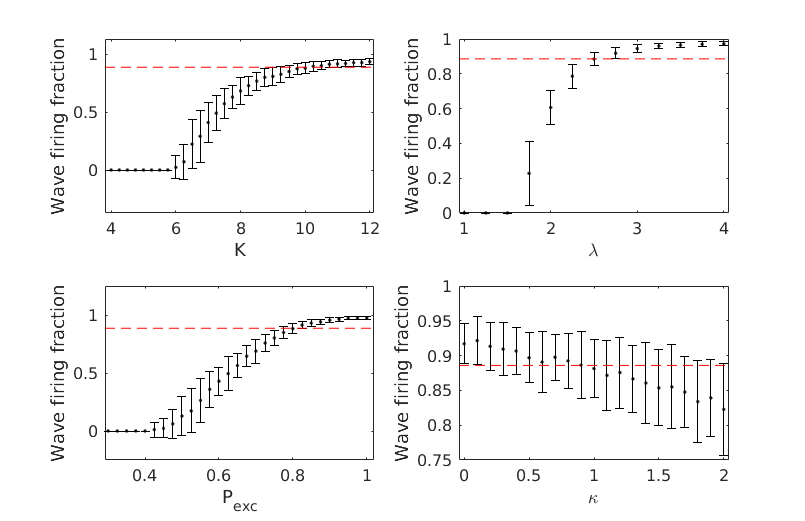
\includegraphics[width=\textwidth]{fig/ParamWaveSim} 
 \rule{\textwidth}{1bp}
 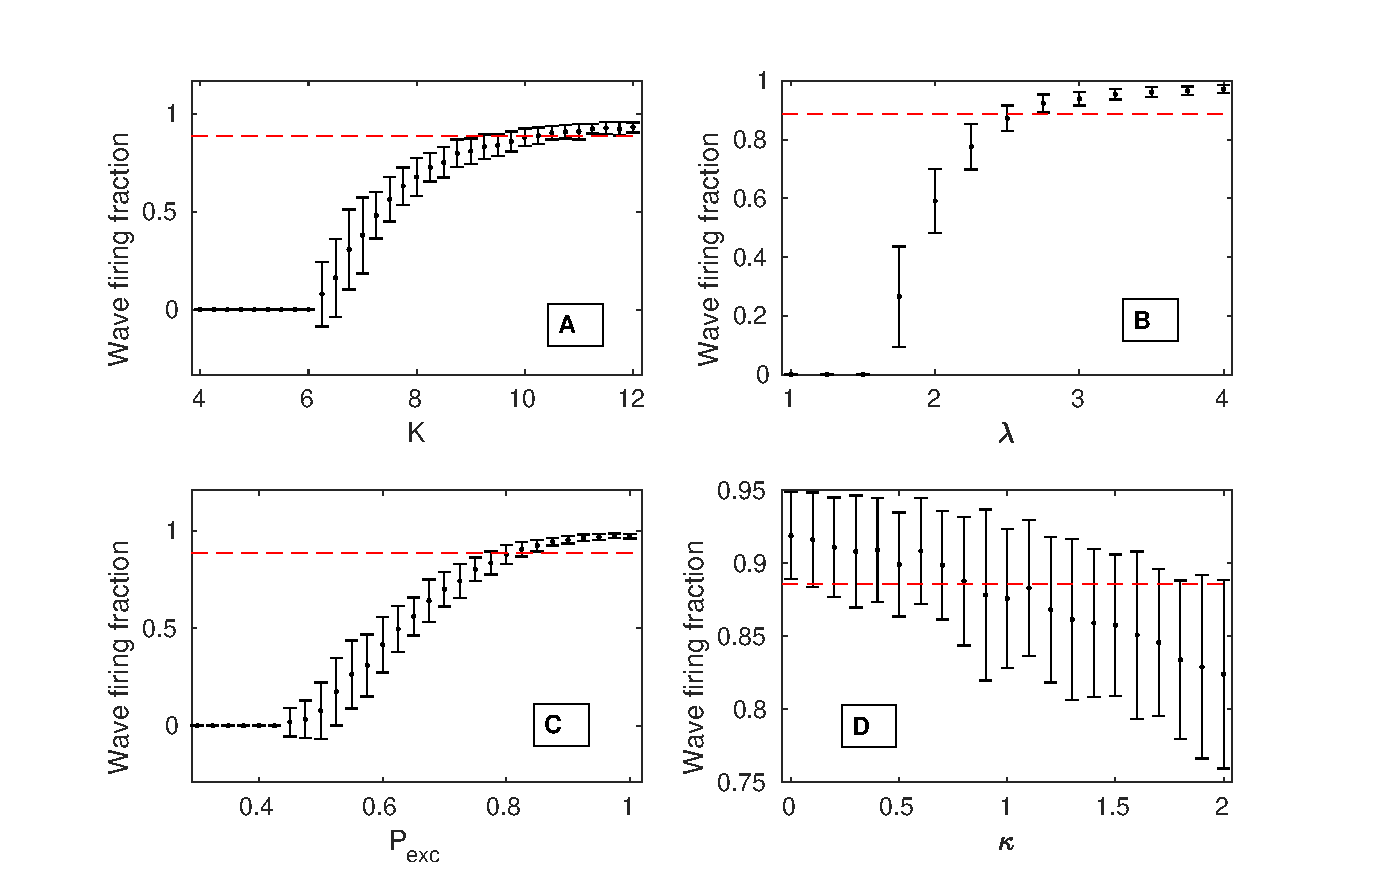
\includegraphics[width=\textwidth]{fig/ParamWaveSim_NoLongConnections}
 \caption{The original results for wave dependence upon model parameters (top) do not substantially change with connections of length $>5$ removed (bottom). }
 \label{fig:wave_parameters_nolongconnections}
\end{figure}
\FloatBarrier

\clearpage
\subsection*{SCE with a larger cross-section}
In section 3.2 we showed that as SCE grow in the X or Y dimension the wave speed increases due to the increased connectivity, but when the average number of connections per neuron were held constant the wave speed was constant.
We further examine these thicker, but still quasi one-dimensional SCE by examining the firing activity of purely one-dimensional sub-columns within the larger SCE (with topology 2x2x100 extracted from the central core of the thicker SCE, away gtom the surfaces, except of course for the 2x2 and 3x3 SCEs).
With the average number of connections held constant, the sub-columns within the larger SCE show similar firing fraction with $K$ regardless of the overall topology (Figure \ref{fig:LargeSCESubcolumns}).
We remark that as the X and Y extents increase, the behavior seems to change from traveling waves to more synchronized firing activity.
This behavior as a function of width suggests that the system dynamics transition from supporting traveling waves to a system that exhibits global synchrony.
\begin{figure}[!htb]
 \caption{ Spike raster plots for complete SCE (A) and one-dimensional sub-colmns (B) for different topologies show similar firing patterns in the sub-columns regardless  of topology. 
           The wave firing fraction (C) measured within the sub-columns show the same dependence on $K$ regardless of the topology.}
   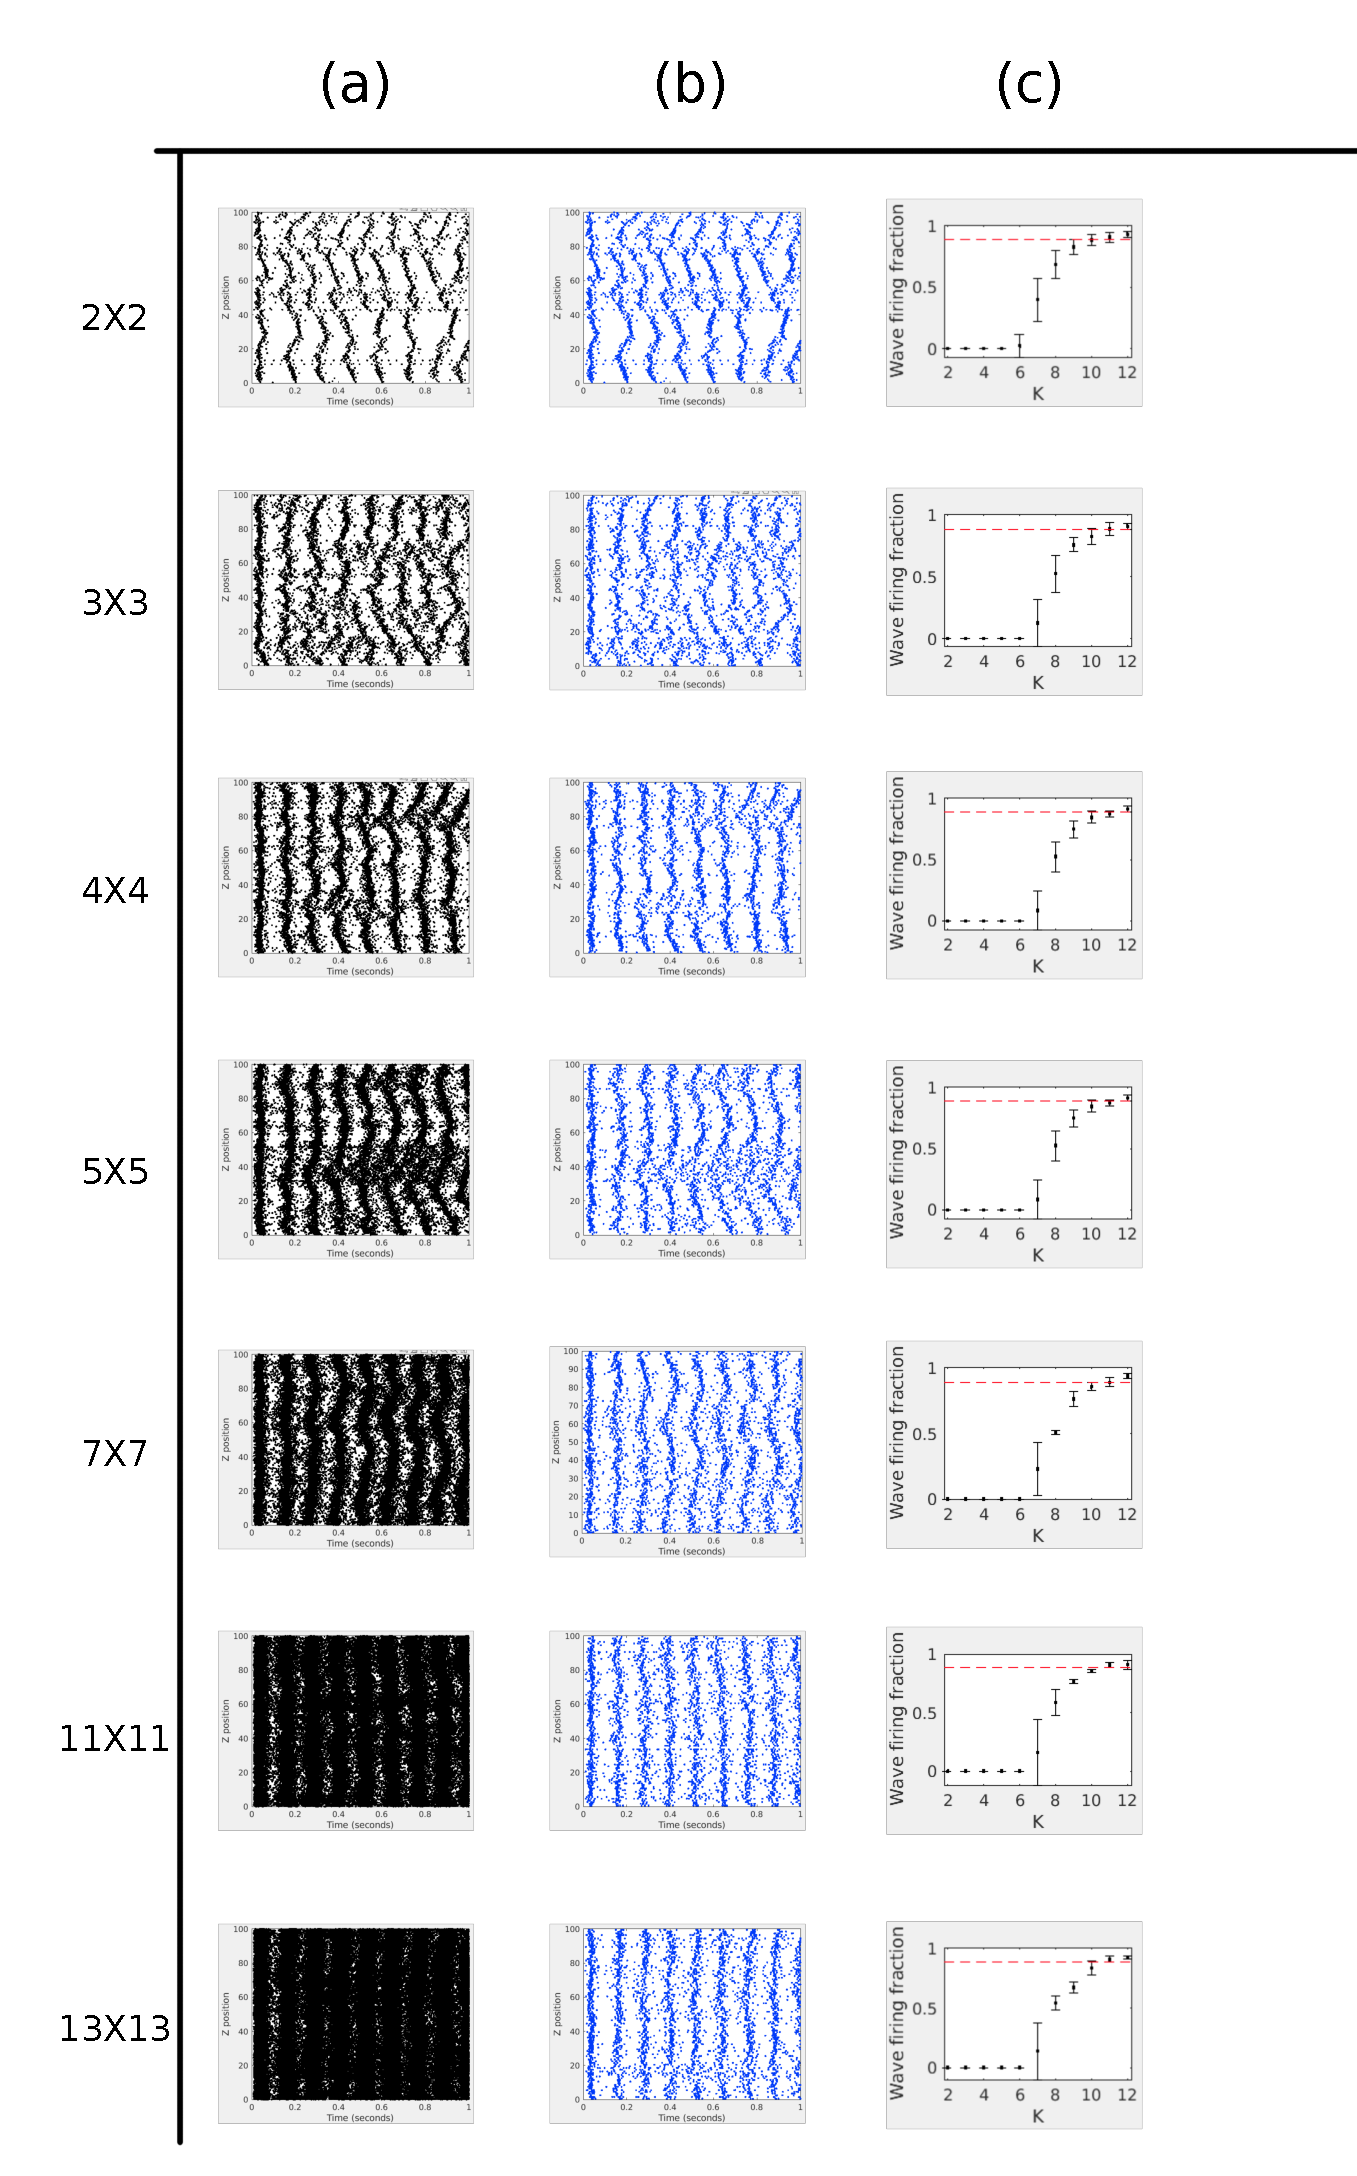
\includegraphics[width=0.75\textwidth]{fig/WaveFractionVsThick}
   \label{fig:LargeSCESubcolumns}
\end{figure}
\FloatBarrier

\color{black}
\end{document}
